In this chapter, 

\section{Flow}

In this section, the general flow of the usage of the visualization application is guided. At the beginning, the blockchain system is empty, and the user can either upload a configuration file or add nodes manually (Figure \ref{fig:start of the application}). The introduction starts with creating nodes and publishing transactions manually, as it is clearer to begin with an simple example.

\begin{figure}[htb]
    \centering
    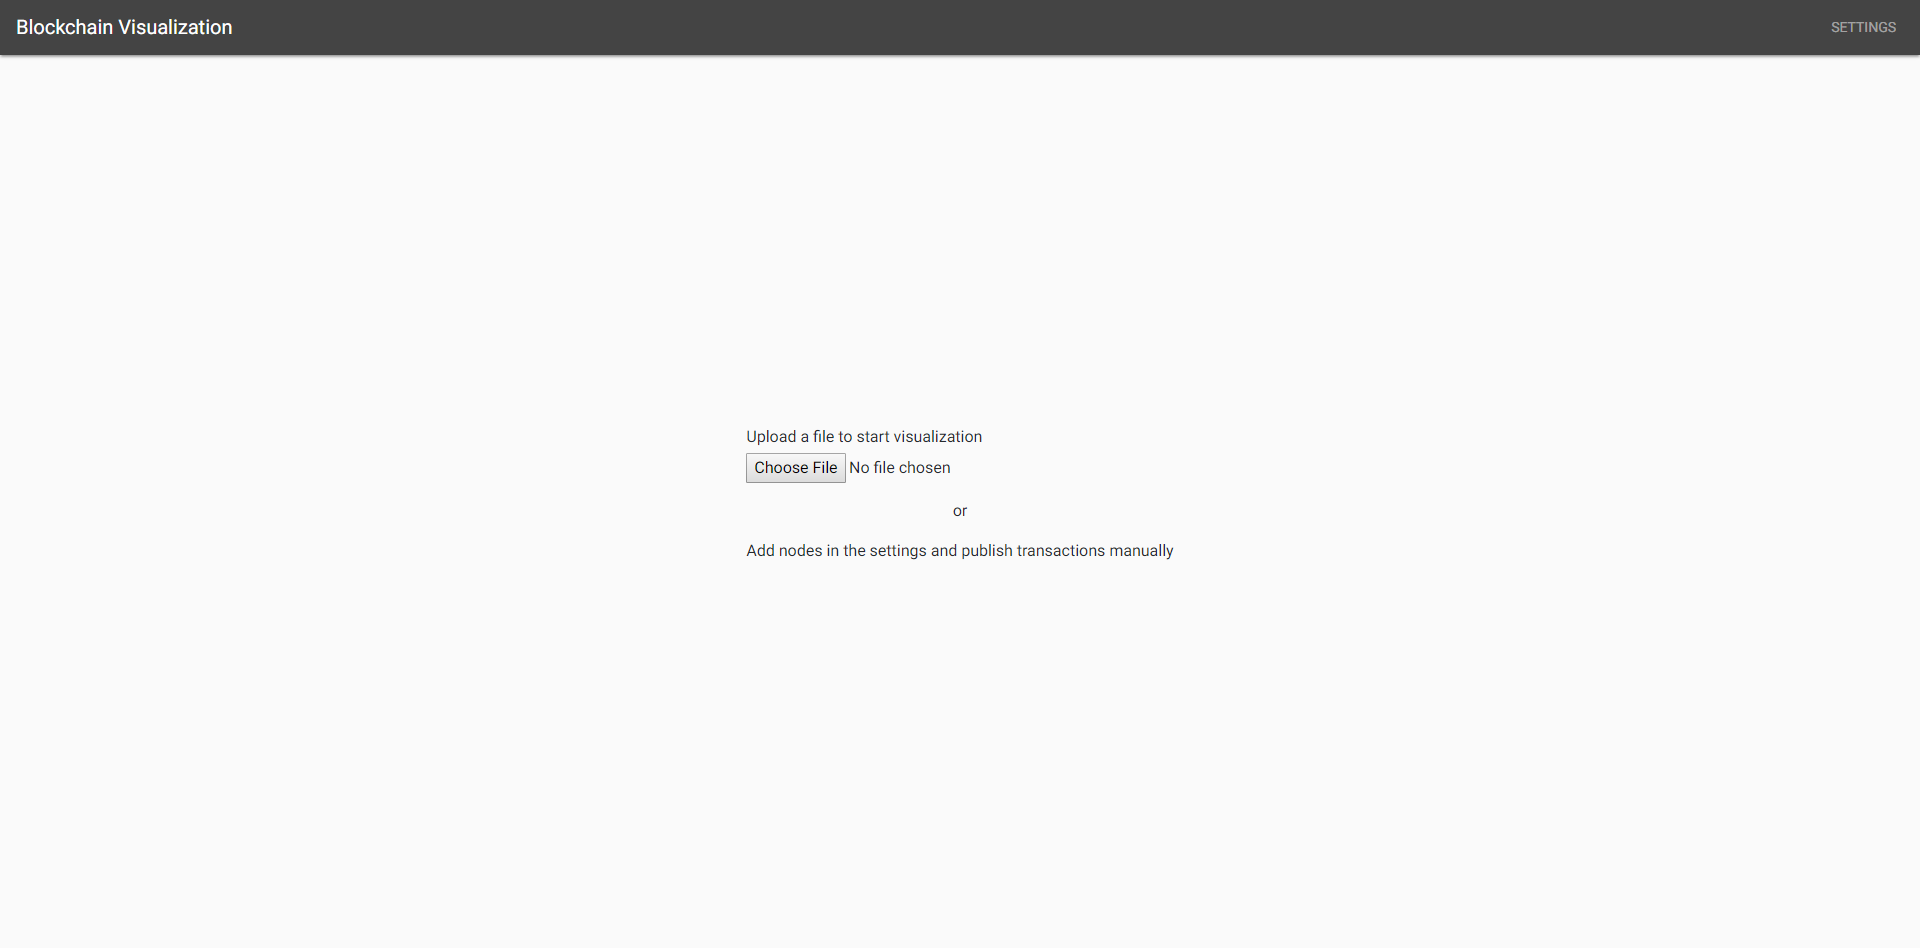
\includegraphics[width=\textwidth]{application_start}
    \caption{Start of the Application.}
    \label{fig:start of the application}
\end{figure}

By clicking the top right button in the navigation bar, the user will be redirected to the settings page, as Figure \ref{fig:settings page} shows.

\begin{figure}[htb]
    \centering
    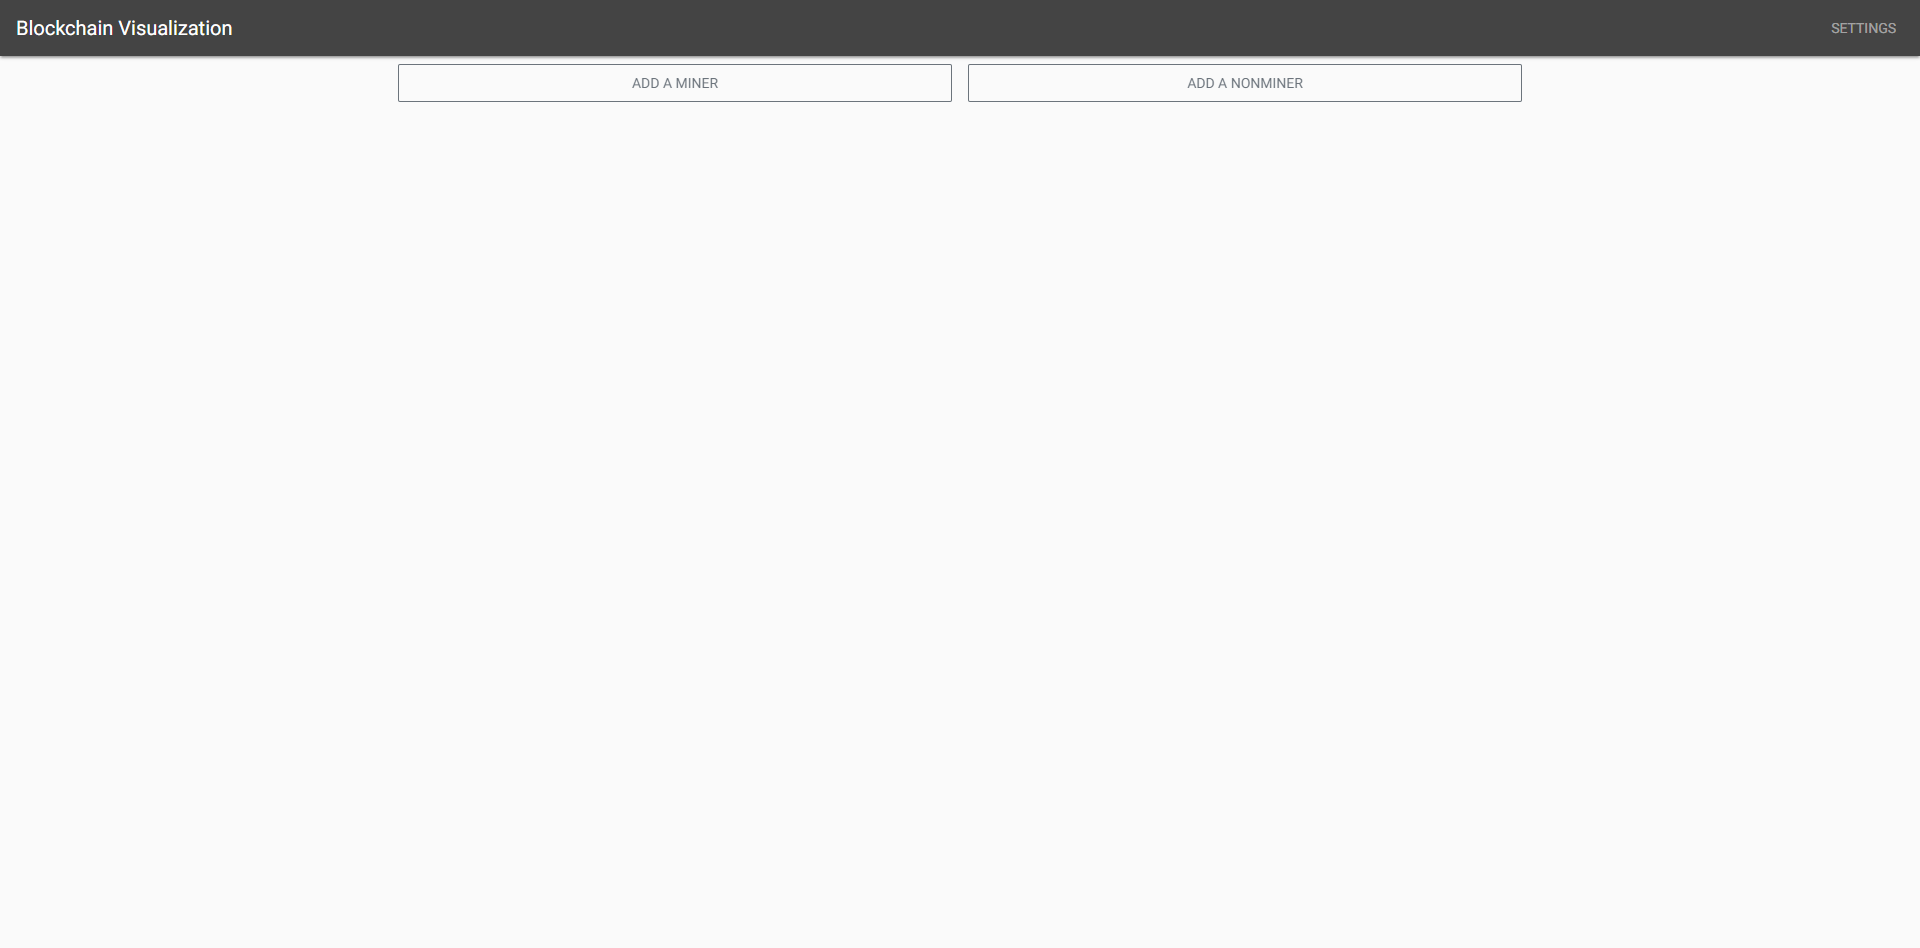
\includegraphics[width=\textwidth]{application_settings}
    \caption{Settings Page.}
    \label{fig:settings page}
\end{figure}

The settings page contains all the nodes that exist on the blockchain network. However, the blockchain system is empty currently, so the settings page is empty. To add a node, the user can click ``ADD A MINER'' button or ``ADD A NONMINER'' button. In this example, we add three miners and two nonminers.

\begin{figure}[htb]
    \centering
    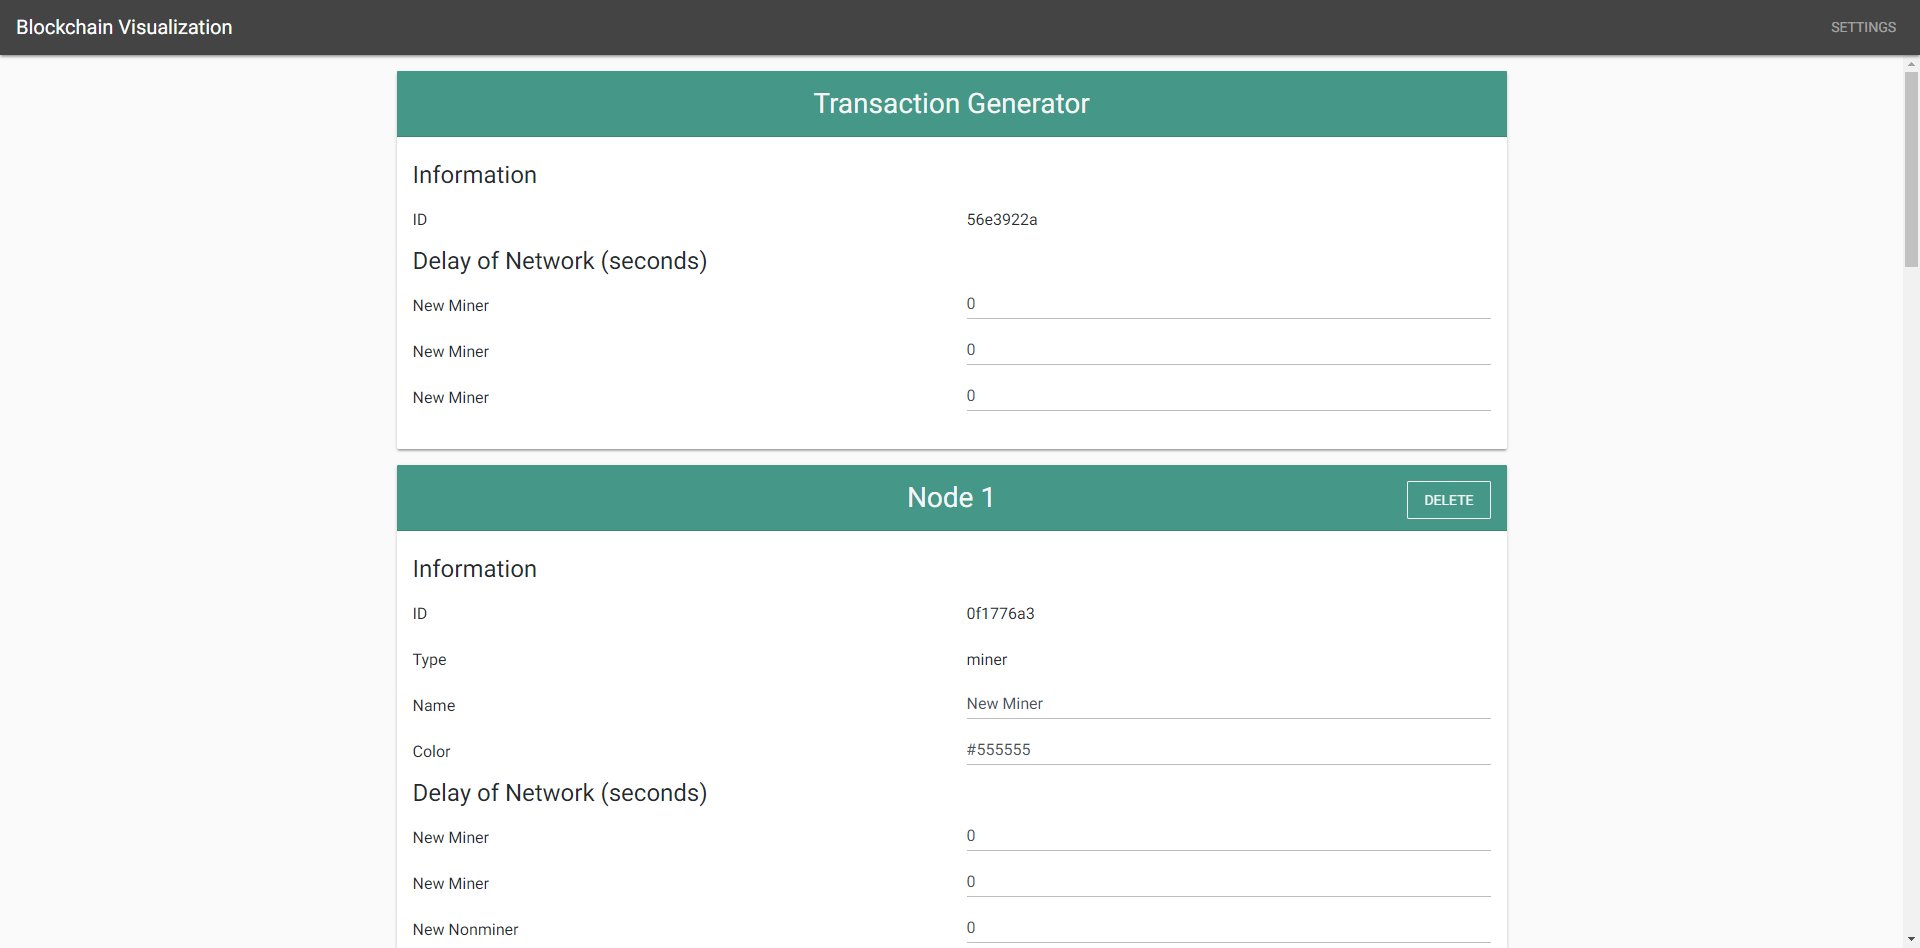
\includegraphics[width=\textwidth]{application_settings_tg}
    \caption{Settings of Transaction Generator.}
    \label{fig:settings of transaction generator}
\end{figure}

After creating nodes, the settings page contains three miners and two nonminers now. Additionally, the transaction generator is added to the blockchain system automatically. In Figure \ref{fig:settings of transaction generator}, the properties of the transaction generator is displayed in the toppest block. The properties contain the ID and the delays to its neighbors.

\begin{figure}[htb]
    \centering
    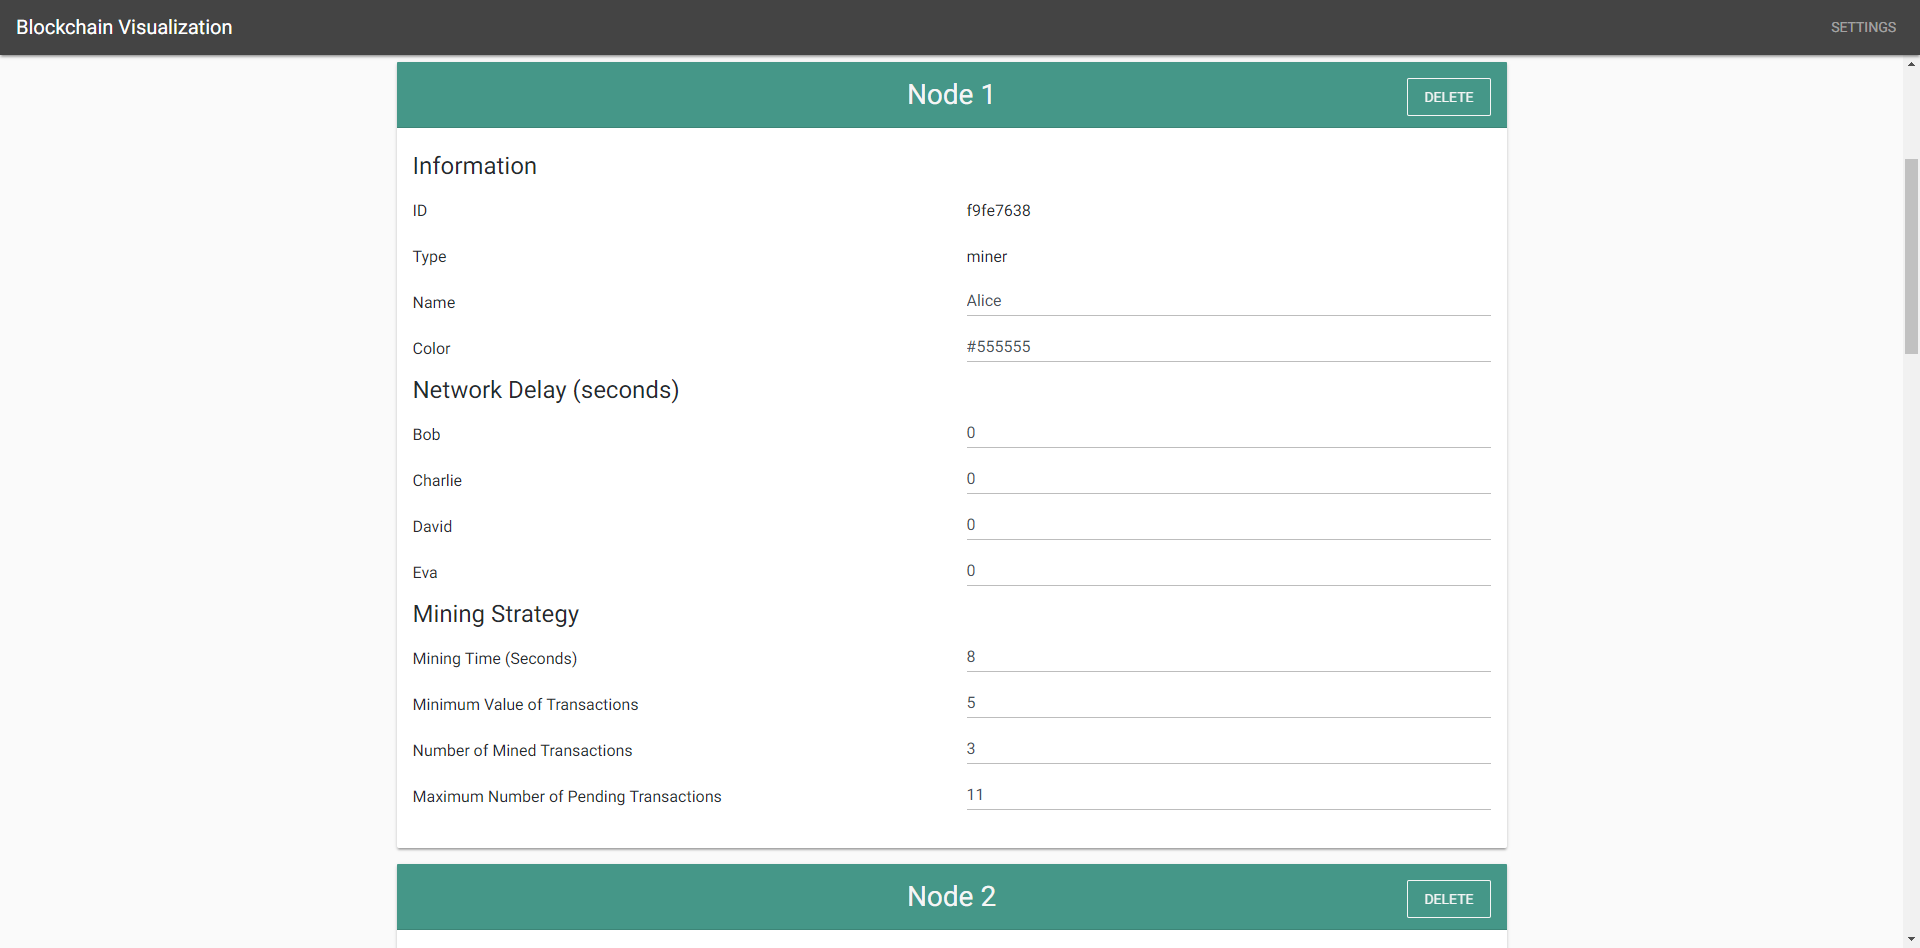
\includegraphics[width=\textwidth]{application_settings_m}
    \caption{Settings of Miner.}
    \label{fig:settings of miner}
\end{figure}

By scrolling down the settings page, the miners that exist in the blockchain system are displayed first. The configuration of the miners can be divided into three parts.

\begin{itemize}
    \item \textbf{Information} \\
        The properties of the miner, including the ID, the name, and the represented color.
    \item \textbf{Delays of Network} \\
        It defines all the delays to the neighbors.
    \item \textbf{Mining Strategy} \\
        This part contains the four parameters that are used for the mining strategy.
\end{itemize}

\begin{figure}[htb]
    \centering
    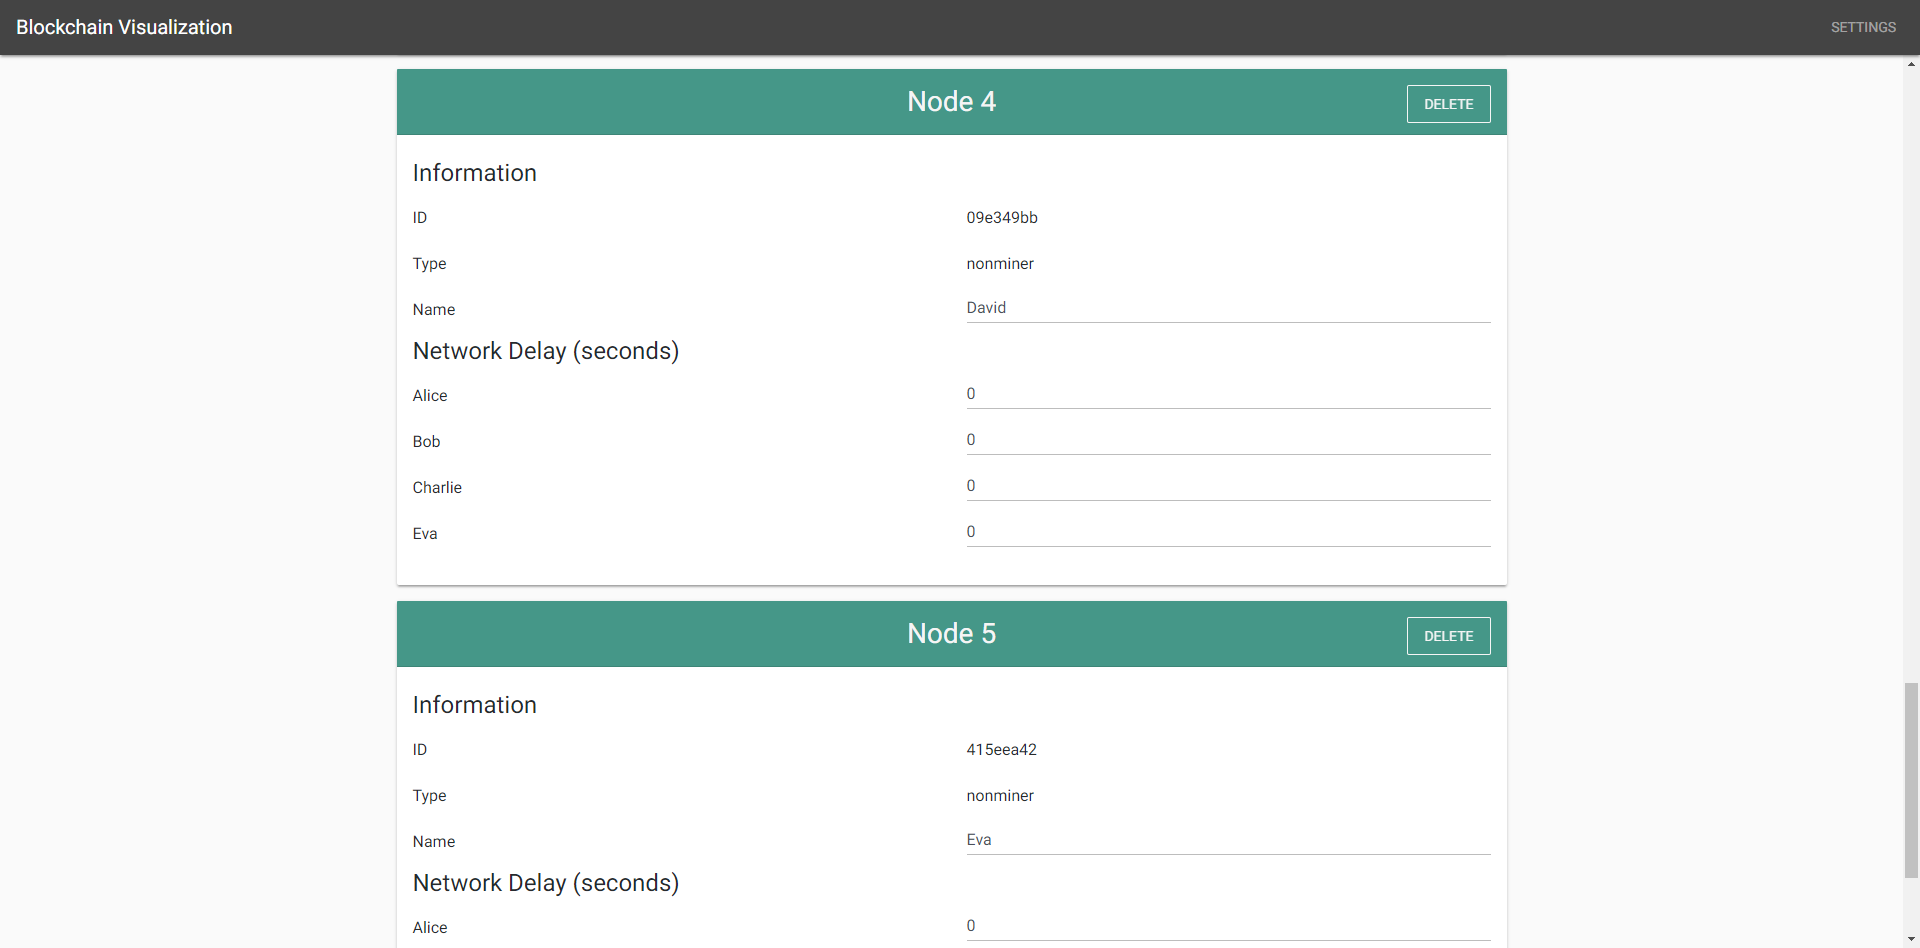
\includegraphics[width=\textwidth]{application_settings_nm}
    \caption{Settings of Nonminer.}
    \label{fig:settings of nonminer}
\end{figure}

The last part of the settings page is for the nonminers. Because nonminers do not mine a block by themselves, the represented color and the parameters of mining strategy are missing here, as Figure \ref{fig:settings of nonminer} shows.

The user can give miners and nonminers nicknames such as Alice, Bob, etc., to make the relationship of the nodes more understandable. The nicknames may not be unique in the blockchain system for the reason that the nodes are recognized by their unique IDs. Moreover, the parameters are updated automatically while the user is typing. All of the parameters are generated randomly at first, so it is better that checking and setting each parameter manually.

In this example, we set Alice (red color), Bob (blue color), and Charlie (green color) as miners, and David and Eva as nonminers. For the mining strategy, we set the following three parameters to the same number for all miners.

\begin{itemize}
    \item Mining Time (Seconds): 1
    \item Number of Transactions to be Mined: 1
    \item Maximum Number of Pending Transactions: 10
\end{itemize}

For the parameters of \textit{minimum value of transactions}, we set 1 for Alice, 5 for Bob, and 9 for Charlie. Hence, Alice is expected to mine blocks faster than Bob and Charlie. For the delays of networks, we set all the parameters to one second.

\begin{figure}[htb]
    \centering
    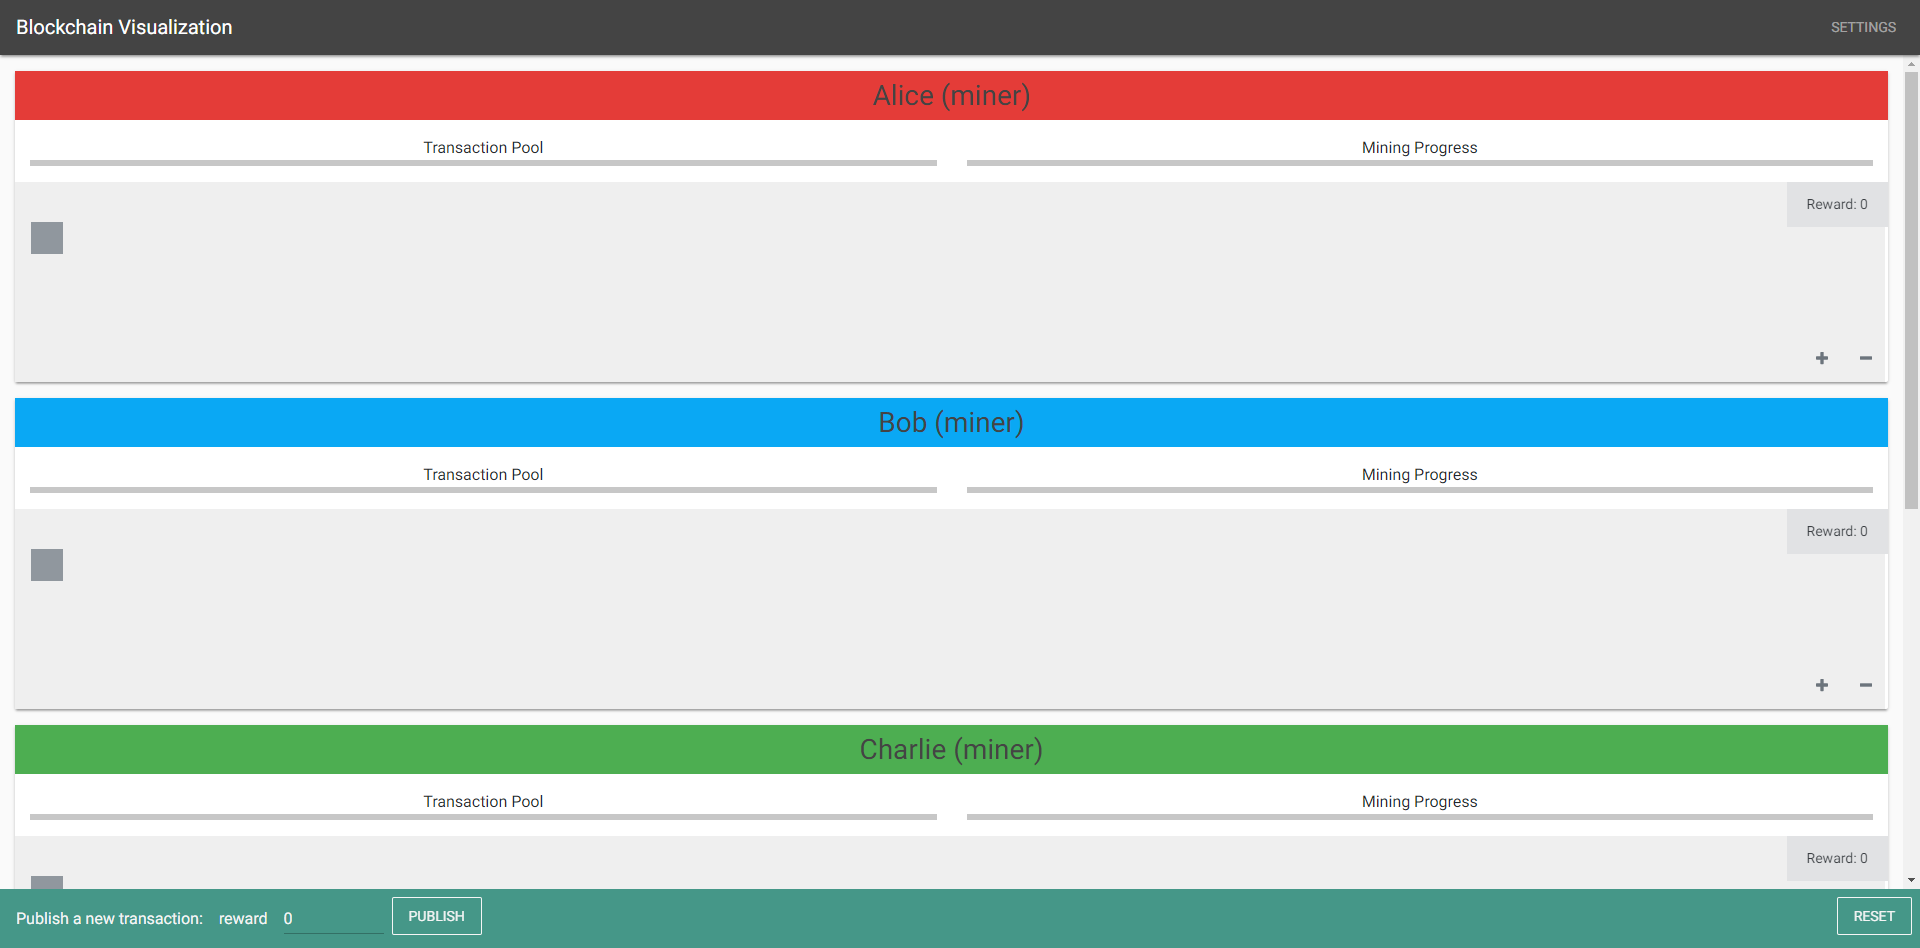
\includegraphics[width=\textwidth]{application_index}
    \caption{Initial status.}
    \label{fig:initial status}
\end{figure}

After finishing the configuration, the user can see the initial status of the blockchain system like Figure \ref{fig:initial status}. Each row represents the visualization of a miner or nonminer. A miner has a colorful head and two progress bars which display the status of the transaction pool and the mining activity. At the bottom of each row, it is the main area for visualizing the blockchain data structure. At the beginning, the grey block represents the genesis block.

\begin{figure}[htb]
    \centering
    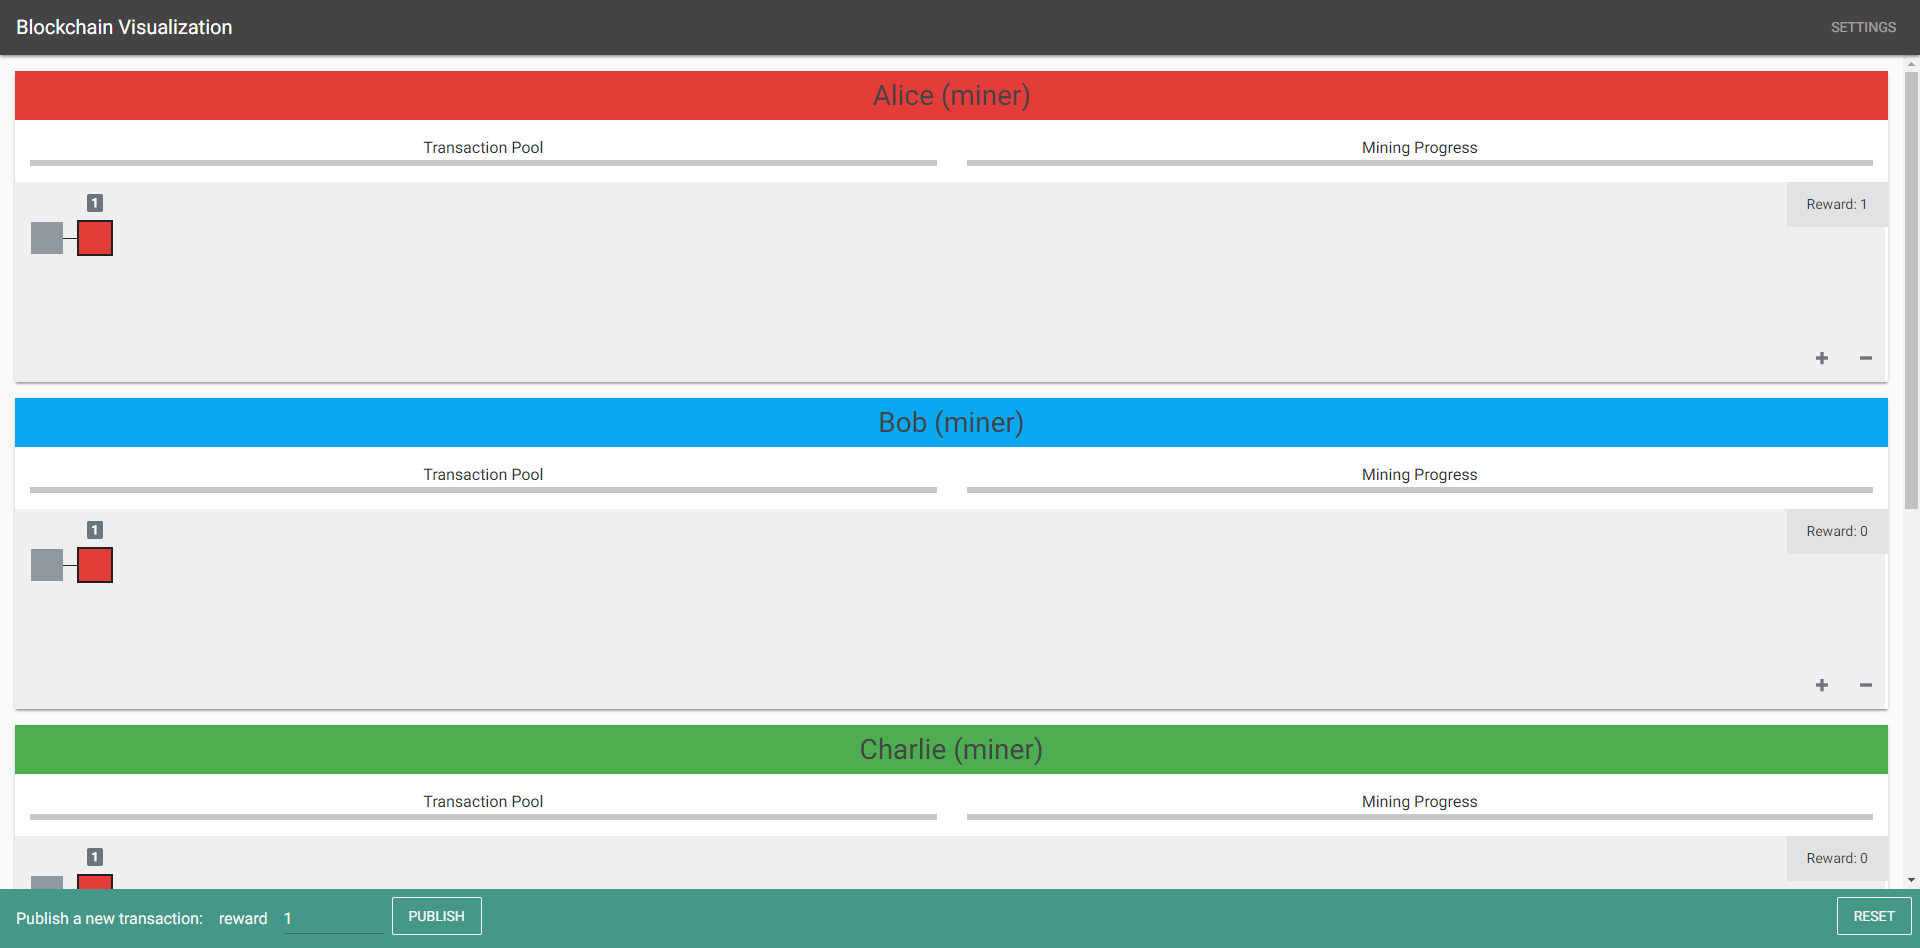
\includegraphics[width=\textwidth]{application_demo1}
    \caption{Alice mined a block.}
    \label{fig:alice mined a block}
\end{figure}

The user can publish a transaction at the bottom area of the screen. By entering a number of the reward, a transaction will be generated by the transaction generator and published. In the first step, we publish a transaction which reward is 1. Hence, it is expected that only Alice will mine a block because the \textit{minimum value of the transactions} is 1 for Alice, and the necessary \textit{number of transactions to be mined} is also 1. The result is showed in Figure \ref{fig:alice mined a block}. Moreover, now Alice's total reward is 1 because she added a block to the longest blockchain successfully.

\begin{figure}[htb]
    \centering
    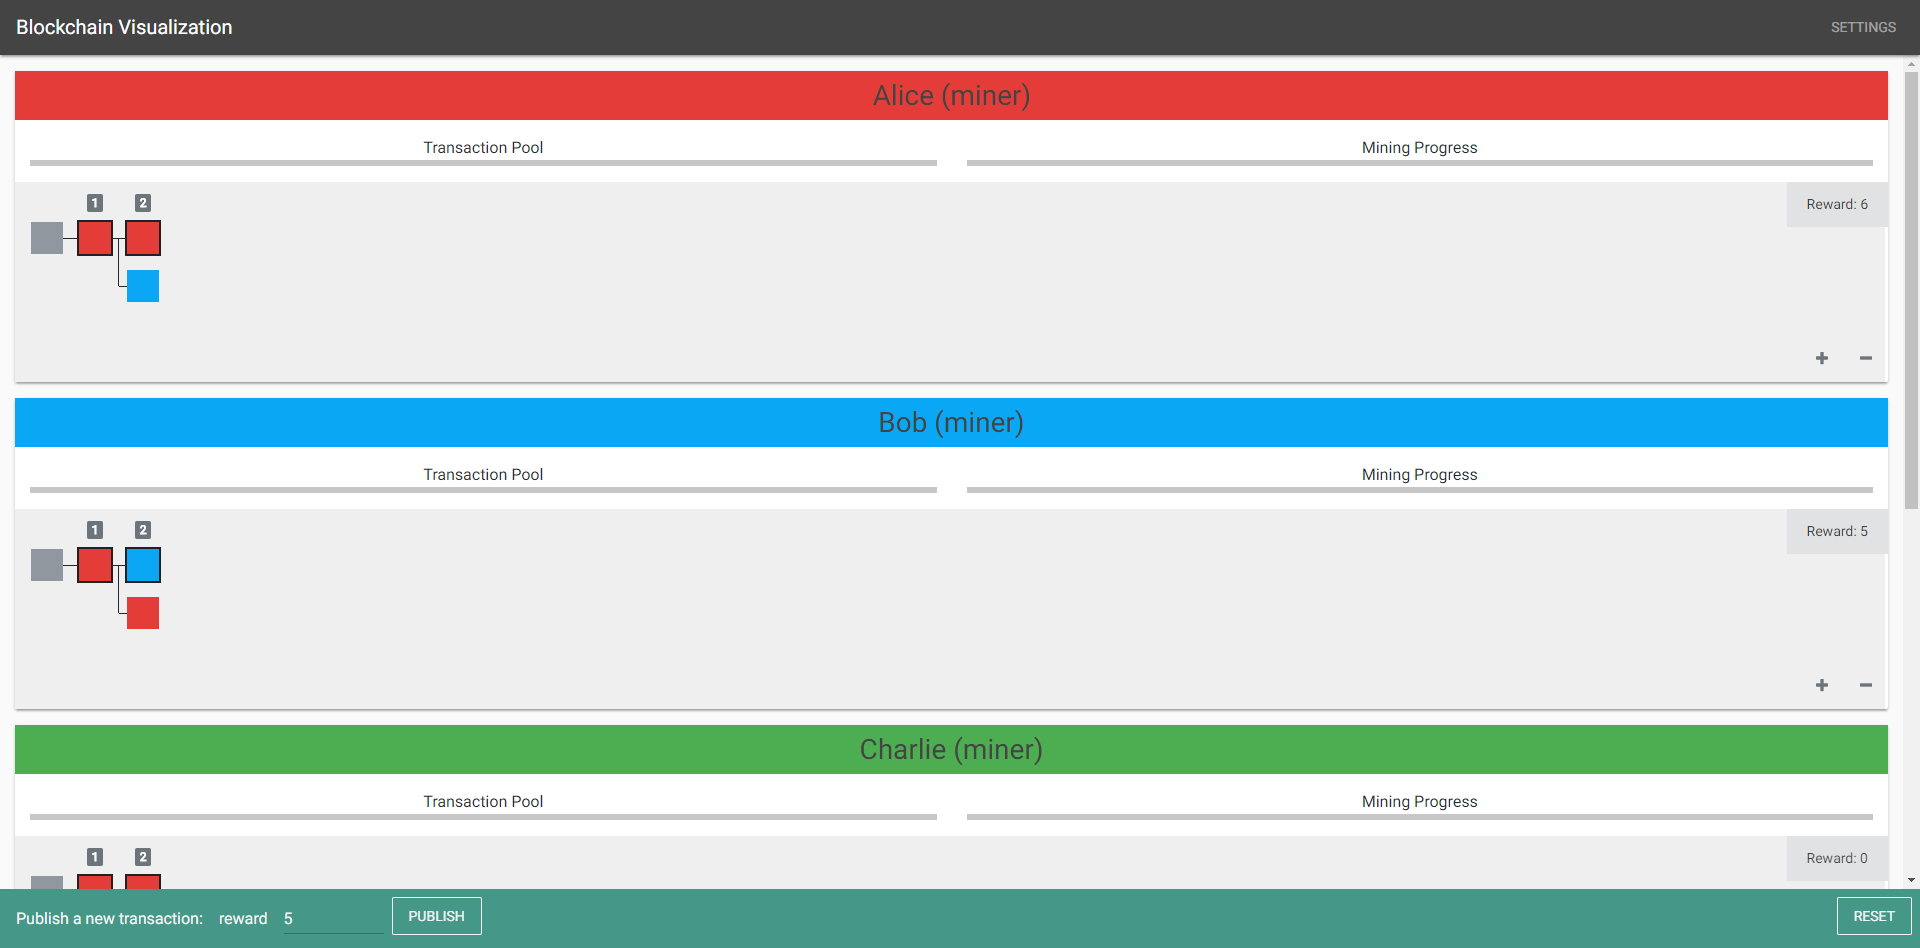
\includegraphics[width=\textwidth]{application_demo2}
    \caption{Alice and Bob mined a block simultaneously.}
    \label{fig:alice and bob mined a block simultaneously}
\end{figure}

In Figure \ref{fig:alice and bob mined a block simultaneously}, it demonstrates that Alice and Bob competed with each other by adding a block at the same time. Because we published a transaction with 3 rewards, Alice and Bob both decided to mine a block according to their mining strategies. As a result, the fork happened for the reason of simultaneous mining activities.

\begin{figure}[htb]
    \centering
    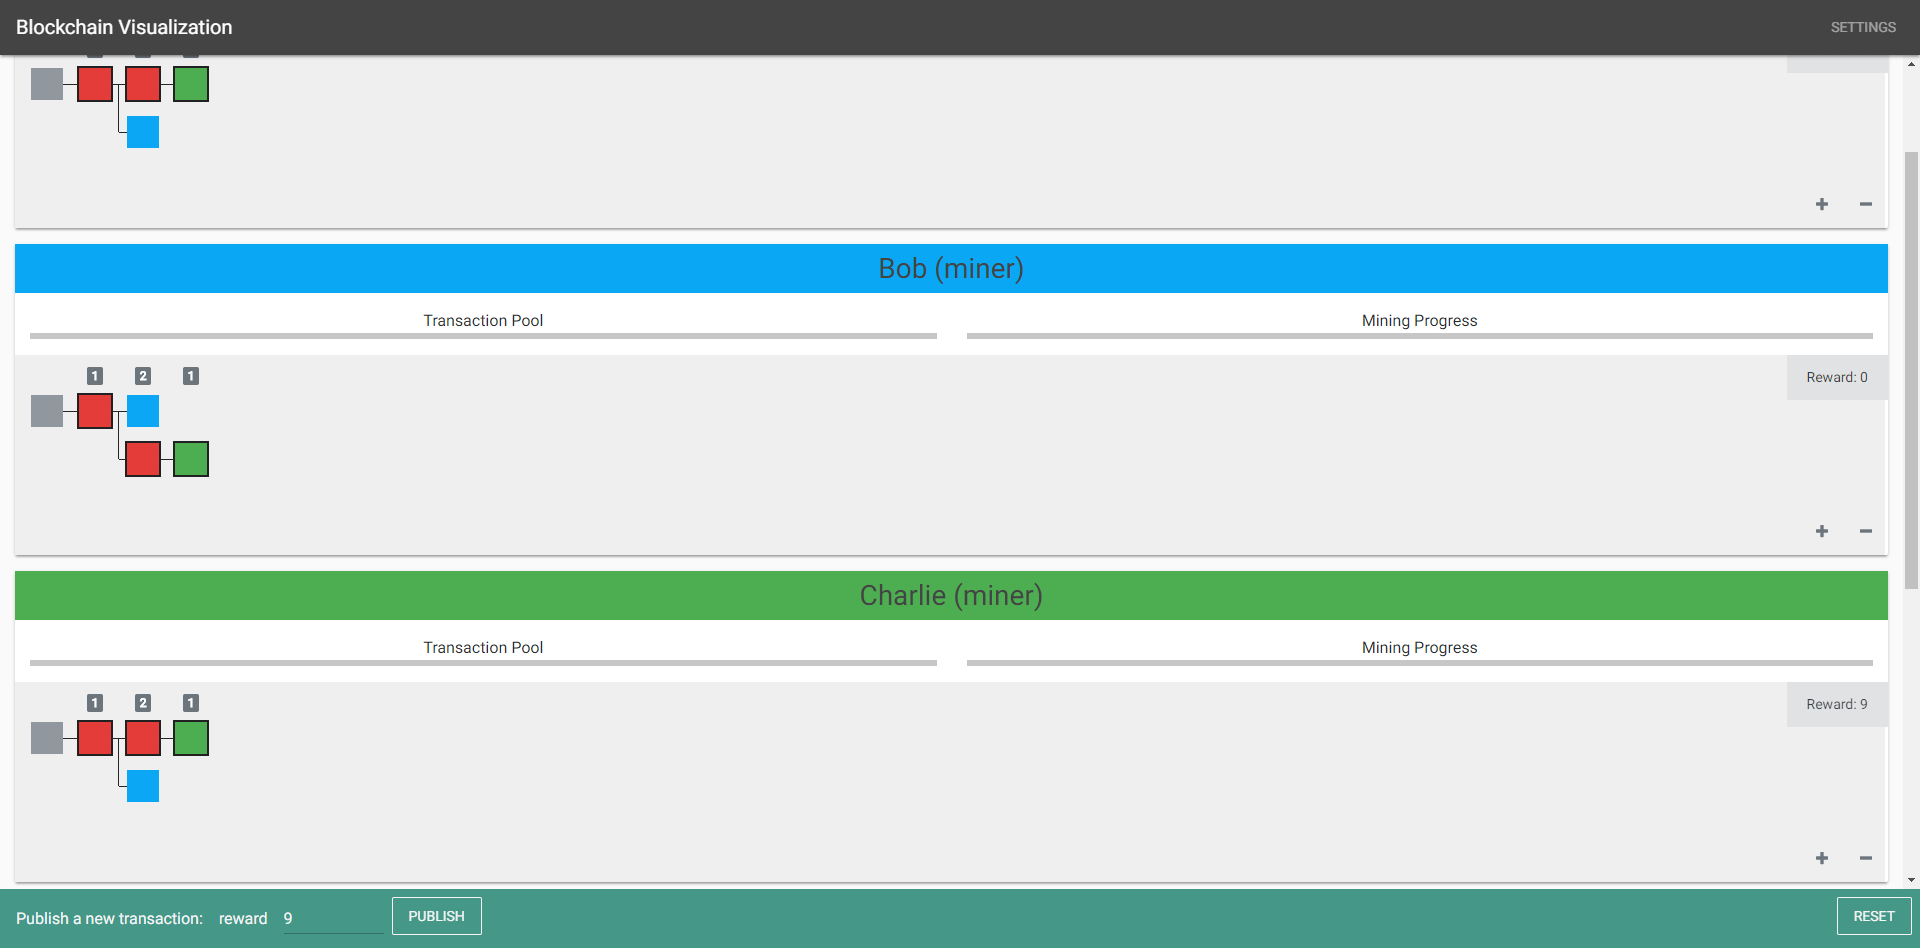
\includegraphics[width=\textwidth]{application_demo3}
    \caption{Charlie mined a block.}
    \label{fig:charlie mined a block}
\end{figure}

In the next step, Figure \ref{fig:charlie mined a block} shows the influence of the mining strategy to the mining processes. We changed the parameters of the mining strategy at first. Thus, Alice's and Bob's parameters of \textit{number of transactions to be mined} were both changed to 2. After that, a transaction with 9 rewards was published. The result was that Charlie mined a block for the reason that it satisfied Charlie's mining strategy. On the other hand, Alice and Bob did not mine a block because of the insufficient number of transactions.

\begin{figure}[htb]
    \centering
    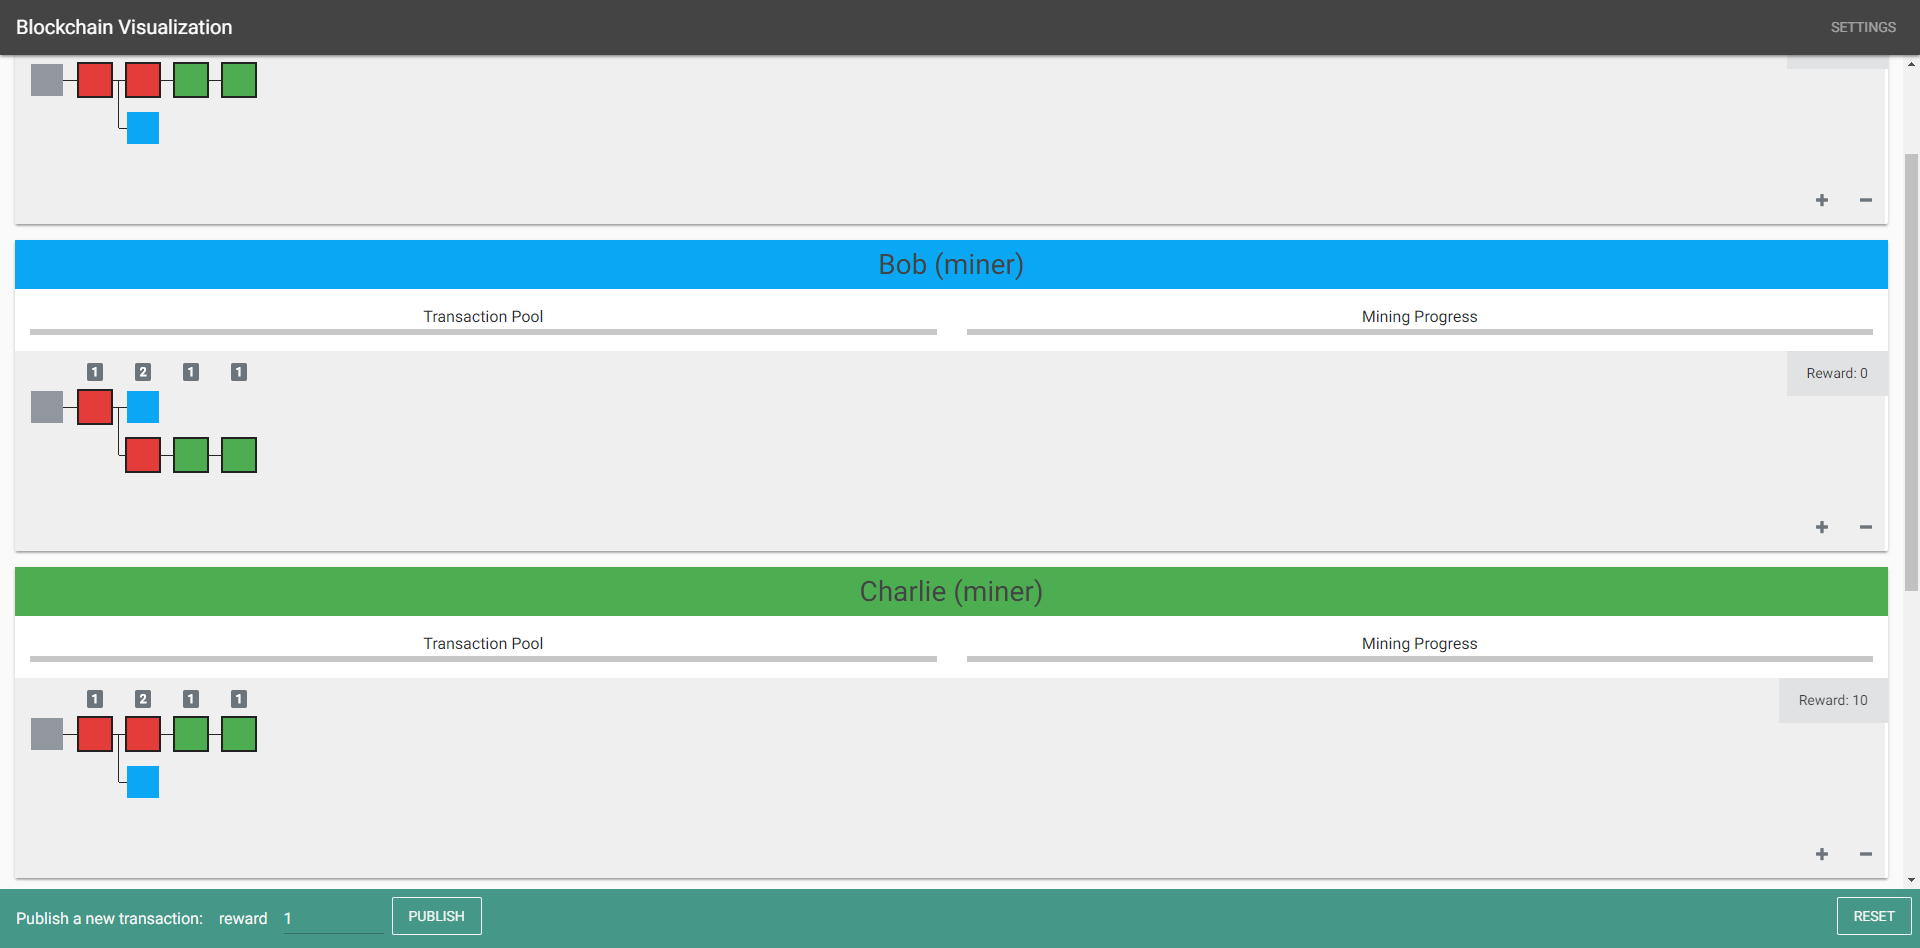
\includegraphics[width=\textwidth]{application_demo4}
    \caption{Charlie mined another block.}
    \label{fig:charlie mined another block}
\end{figure}

Finally, Figure \ref{fig:charlie mined another block} shows the process of selecting candidate transactions. Fist, Charlie's parameter of \textit{minimum value of transactions} was set to 1, and then we published a transaction with 1 reward. The result was that Charlie mined a block after about 8 seconds due to the process of selecting candidate transactions. Normally, a miner starts to select candidate transactions in every second, and the privileges of transactions that are not selected were added by 1 each time. Consequently, the value of the published transaction was becoming 9 after 8 seconds, and it satisfied Charlie's mining strategy.

During the mining processes, the following auxiliary information in the visualization is also helpful and dynamic.

\begin{itemize}
    \item \textbf{Progress bars for the transaction pool} \\
        It displays the level of capicity of the transaction pool.
    \item \textbf{Progress bars for the mining status} \\
        It presents the mining activities in real-time, i.e., how much time is remaining for solving a puzzle.
    \item \textbf{Number of total rewards} \\
        It displays the caculation of the total rewards that belongs to the miner.
    \item \textbf{Number of forks} \\
        On the top of each fork, there is a number that represents the number of forks.
\end{itemize}

Additionally, the user can drag the visualization area to move the blockchain data structure, and zoom in and out by clicking the plus and minus buttons on the bottom right side.

\section{Configuration Files}

To replay the same visualization of blockchain processes, we can define the configuration of the blockchain system in a file and upload it to the application as in Figure \ref{fig:start of the application}. The configuration file is composed of the following three parts.

\begin{itemize}
    \item the properties and the parameters of the mining strategy of nodes
    \item the network delay between each node
    \item the transactions that will be published through the network
\end{itemize}

In Table \ref{}, 


The file is in JSON format, and the file is uploaded to initialize the blockchain system at the beginning.

First, for nodes, it is important to define a unique transaction generator at first, and then it is followed by miners and nonminers. After that, a list of delays between each node is defined. As mentioned before, the transaction generator only connects to miners, and miners and nonminers connect with each other. In the last part, it contains a list of transactions with rewards and the time when the transaction will be published after the starting of the blockchain system.